\chapter{System Design} \label{chap:System Design}
In this chapter, we discuss the high-level requirements for the system to be developed in this thesis and the system architecture is explained in detail. 
At the end of the chapter, we will discuss the design choices and system features.

\section{System Requirements}
The requirements for the system developed in this thesis are analyzed according to the idea that the dependency graph visualization and history, improve the debugging process of an application based on reactive javascript libraries. We identified following requirements expressed in terms of functionalities available to the end user.

\leavevmode
\\
\textbf{Availability}
\\
The new system should seamlessly work and should be easily installable. Therefore, in order to reach many web developers, an extension for Google Chrome is being developed. 

\leavevmode
\\
\textbf{Visualization of the Dependency Graph}
\\
While debugging, the developer should be able to see the dependency graph generated based on the developers' code. For the selected variable, all the dependents and dependencies of the variable should be shown in the graph, so that the developer understands the overview of the system. 
When the new values are generated, the graph should be automatically updated.

\leavevmode
\\
\textbf{Visualization of the History of the Dependency Graph}
\\
Once the graph is generated, the developer should be able to have a look at the graph at any arbitrary point in time. Thus, the whole history of the evolution of the graph can be visualized. It should also be possible for a developer to easily navigate through the time and observe the events such as node creation, node updates, dependency updates etc.

\leavevmode
\\
\textbf{Querying the History of the Graph}
\\
Depends on the size of the application, the size of graph grows. For large applications, it is not feasible to manually navigate through each step of the graph evolution. Therefore, a query language should be developed such that it makes easier for the developer to jump to specific points/events in the history. For example, the system should be able to jump to a specific point at which a node is created or updated.

\leavevmode
\\
\textbf{Breakpoints}
\\
Sometimes developer wants to halt the execution of the program by setting breakpoints at specific events. Our system should also provide developer an option to set breakpoints. For instance, it should be possible to set a breakpoint which is hit when a specific node is created or evaluated. 

\leavevmode
\\
\textbf{Helpers}
\\
System provides following additional features to the developer.

\begin{itemize}
	\item Search node by name in dependency graph.
	\item Pause or resume logging all values to the graph.
	\item Exclude selected nodes from logging values to the graph.
	\item An option to chose whether developer wants to print all the logged values to the console.
	\item Show dependents and dependencies of the selected node.
\end{itemize}

\section{System Architecture Overview}
The overall system design is illustrated in Figure~\ref{fig:system-design}. There are two system components: one is chrome extension which provides extended debugging functionality for reactive applications and another one is client code which needs to be debugged. The general interaction between client code and extension is shown in the figure~\ref{fig:system-design}. 

\begin{figure}[!h]
	\centering
	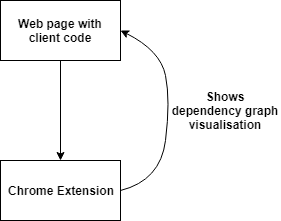
\includegraphics[scale=0.6,trim=0 0 0 0]{images/system-design.png}
	\caption{Overview of system design}
	\label{fig:system-design}
\end{figure}

The detailed system architecture is depicted in figure~\ref{fig:system-architecture}. The application is written using reactive javascript libraries(RxJS/BaconJS). Analyzer is a core component of the system. It helps the extension to catch all the events happening at both the libraries. In the current implementation, we support two reactive javascript libraries, RxJS and BaconJS. Analyzer analyzes all the events and passes the relevant information further to Chrome Reactive Inspector(CRI) panel. The information received by the panel is then stored in browser storage and also displayed as a dependency graph. CRI stores in-between steps or data to browser storage which helps developer for back in time debugging.

\begin{figure}[!h]
	\centering
	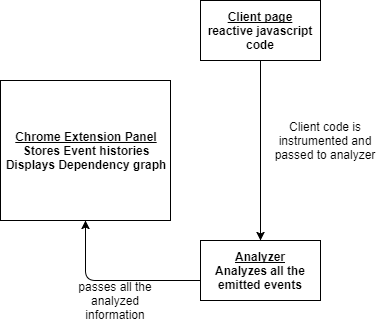
\includegraphics[scale=0.6,trim=0 0 0 0]{images/system-architecture.png}
	\caption{System Architecture}
	\label{fig:system-architecture}
\end{figure}

\subsection{Analyzer}
As we said earlier, Analyzer is the main building block of our system. It receives all the events and analyzes them. We will now look into how Analyzer is designed in detail.

RxJS library does not provide any interfaces to the developer for debugging purpose yet. But BaconJS provides the user an interface in the form of \textbf{Bacon.spy} method. Using this method, the developer can catch all the events emitted by clients' BaconJS code. Keeping these in mind, we designed Analyzer as shown in the figure~\ref{fig:analyzer-design}. 

\begin{figure}[!h]
	\centering
	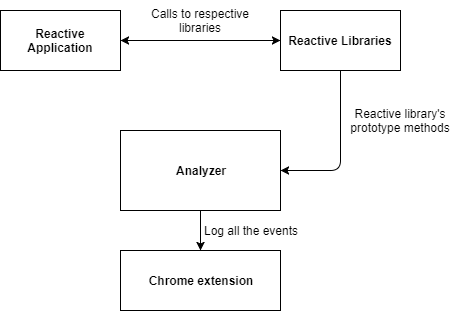
\includegraphics[scale=0.6,trim=0 0 0 0]{images/analyzer-design.png}
	\caption{Analyzer Design}
	\label{fig:analyzer-design}
\end{figure}

Here, we intercept and rewrite the required functions of both the libraries using prototype\cite{prototype}. Every object in javascript has an internal property called Prototype. Using this property, we are overriding required function calls of both libraries. We capture the required information and handover the call to original library call for further computations. Overriding all the function calls is not feasible and scalable. We observed that calls to various operators returned respective new observables. For instance, map operator returns \textit{MapObservable} in RxJS. All types of observables call their respective subscribe functions which internally calls parent subscribe method. Thus, we only override parent subscribe method instead of individual subscribe methods. 

\section{System Architecture Details}
\subsection{Dependency Graph Visualization}
As explained earlier, dependency graphs help user visualize reactive applications. Each time-changing value is a node in the graph and a directed connection between two nodes if one node depends on another node. Consider the following RxJS code snippet for example. 
\begin{lstlisting}[language=JavaScript, caption=RxJS code example, label={lst:rxjs-code-example}]
var shortName = name.map(name => name.toLowerCase())
.filter(name => name.length < 5);

var bmi = weight.combineLatest(height, (weight, height) =>
Math.round(weight / (height * height * 0.0001))
);

var fullInfo = shortName.combineLatest(bmi);
\end{lstlisting}

In the above example, in Line 1, variable \textit{shortName} depends on variable \textit{name}. Similarly at Line 4, \textit{bmi} depends on both \textit{height} and \textit{weight}, at Line 8 \textit{fullInfo} depends on both \textit{shortName} and \textit{bmi}. The figure~\ref{fig:rxjs-dependency-graph-example}, how dependency graph looks after modeling it. This gives a very good overview of the reactive system and especially of the dependency therein. This should be of great help for developers to understand and analyze the reactive applications. 

\begin{figure}[!h]
	\centering
	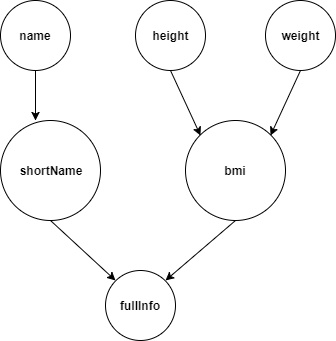
\includegraphics[scale=0.5,trim=0 0 0 0]{images/rxjs-dependency-graph-example.png}
	\caption{RxJS Dependency Graph Example}
	\label{fig:rxjs-dependency-graph-example}
\end{figure}

\subsection{Navigating through the Dependency Graph History}
The visualization of a graph is not only updated whenever an event occurs, but it also stores each stage when it changes. This gives the developer a possibility to navigate through the whole history. The developer can navigate through the history in following ways:
\\
\textbf{History Navigation}
\\
One way is to simply use back and forth buttons provided, which jumps to the point in time directly before or after the current point of time.
\\
\textbf{Direct Access}
\\
History navigation may not be practical for application with large histories. The developer should be able to drag the slider and thus quickly jump to the desired point in time.
\\
\textbf{History Queries}
\\
A third and last option is to navigate through the history using provided query language. By entering valid queries, the developer can directly jump to the respective points in time when these events happened.

\subsection{Breakpoints}
In traditional debuggers, breakpoints are based on specific line or conditions. A breakpoint hits and halts the execution of program each time the code reaches specific line or encounters specific condition evaluates to true. These breakpoint type does not really fit well into the RP approach. Hence, RP specific breakpoints should be developed. They reuse the developed query language. The developer can enter a query, start to debug the application and the debugger will halt the execution each time the query matches. For instance, if developer enters a query \textit{NodeCreated[NodeId, 1]}, the debugger will halt the execution when a node with Id 1 is created. 

\subsection{Chrome extension}
In this thesis, we are implementing a debugger in the form of an extension to Google Chrome DevTools. With the help of chrome APIs, we can add more debugging capability to our extension. The extension adds a new panel to DevTools which provides all the features mentioned so far and also adds an options page where a user can use optional features. The same extension can be further extended and adapted to support other browsers like Mozilla Firefox\cite{firefox}.

\subsection{Scoping and other features}
The Jalangi framework, which we discussed earlier, instruments the given javascript code. It is performance hindering if we are instrumenting all other code which is not RxJS. So we provide scoping feature where a user can mention the file name to be instrumented. 
Another feature is, a user can search any existing node by name. This feature is useful when the dependency graph is large. The user can also figure out dependents and dependencies of any given node. As optional features, a user can exclude nodes to log events to the graph, can choose whether to log all the values to console. 

\subsection{Chrome Storage}
The Google chrome provides data storage facility to manage data for specific requirements\cite{chrome-storage}. There are options of local storage, session storage and an HTML5 storage available in chrome. The data is stored in the form of key-value pair. Local storage is persistent and has no expiration until the user deletes it explicitly. On the other hand, session storage is persistent only for current browser session and is erased when a browser is closed. We use local storage in our extension to store the data such as file name used for scoping feature, list of breakpoints, list of nodes to be excluded from logging events to the graph.

